\chapter{High-rate motion data pre-integration}
\label{chp:preintegration}
\minitoc
\bigskip


Sensor modalities available on robotic platforms display a great variety in the rate at which measurements are acquired. For instance, 
a camera may record images at 33Hz while an IMU may be updated at 1kHz. In the context of Factor Graph estimation, this creates a challenge since residuals
are defined between \keyframes\ selected at a relatively low frequency. One needs to integrate measurements from these high-rate sensors between \keyframes\,
which is not trivial in general.

In this chapter, we first describe the example of the integration of IMU measurements which motivates the development of the pre-integration theory \cite{lupton-09,forster2017-TRO}.
We then express this pre-integration in more abstract mathematical terms so as to generalize it to other high-rate sensors \cite{atchuthan-18-thesis}. 
Then, we describe a possible reformulation of the original IMU-preintegration algorithm \cite{forster2017-TRO} by exploiting a new Lie group that we 
proposed in \cite{fourmy2019absolute}. We conclude the chapter with a discussion of related works.

  
\section{A motivational example: IMU integration for graph optimization}
\label{sec:imu_preint_motivation}

In this section we will introduce the IMU measurement model and explain why a naive integration of these measurements in the world frame does not immediately
lead to a viable factor. We will then introduce the observations that lead to the development of the so-called IMU pre-integration algorithm by Lupton \cite{lupton-09}.

Let us consider the estimation of a robot base state comprised of its pose and velocity in the world frame,
%
\begin{equation}
    \bfx = [\posi{W}{WB}, \vel{W}{WB}, \Rot{W}{B}]
    \triangleq 
    [\bfp, \bfv, \Rot{}{}].
\end{equation}

We make several hypothesis. We neglect effects due the rotation of the Earth by assuming 
that our world frame (which is fixed \wrt the ground) is an inertial frame. This is a common simplification in robotics scenarios \cite{forster2017-TRO}. 
Without loss of generality, we assume that the IMU frame is identical to the base frame in the following developments.

Among available sensors, the IMU measurements are known to be noisy, biased, and affected by the gravity,
%
\begin{equation}
    \begin{split}
    \angvelm{}{} &= \angvel{B}{WB} + \bias_{\angvel{}{}} + \noise_{\angvel{}{}} 
    \\
    \accm{}{}    &= \Rot{B}{W} \grav + \acc{B}{WB} + \bias_{\acc{}{}} + \noise_{\acc{}{}} 
    \end{split}.
    \label{eq:imu_meas_model}
\end{equation}
    
Other sensors can help estimate IMU biases $\bias \triangleq [\bias_{\acc{}{}}, \bias_{\angvel{}{}}]$ that are thus included in the estimator state.


Once the IMU has been started, these biases may change over time, more or less slowly depending on the quality of the IMU. This change is can be modeled 
as a random walk, which is close to the observed behavior for reasonably short periods of time \cite{hussen2015low}.
A dynamical model based on strapdown integration of IMU measurements can then be derived.

\begin{align}
    &\dot{\posi{}{}} = \vel{}{} \\
    &\dot{\vel{}{}} = \acc{W}{WB} \\
    &\dot{\Rot{}{}} = \Rot{}{} [\angvel{B}{WB}]_{\times} \\
    &\dot{\bias}_{\bfa} = \noise_{\bfa} \\
    &\dot{\bias}_{\angvel{}{}} = \noise_{\angvel{}{}} \\
    \label{eq:imu_dyn_conti}
\end{align}

Introducing the measurement equations \eqRef{eq:imu_meas_model} in continuous dynamics \eqRef{eq:imu_dyn_conti} and using a zero order hold
explicit Euler integration scheme during $\dt$ results in the discrete dynamics:

\begin{equation}
    \begin{split}
    \Rot{}{}^{k+1}  &= \Rot{}{}^{k}\Exp((\angvelm{}{}^k - \bias_{\angvel{}{}}^k - \noise_{\angvel{}{}}^k)\dt)
    \\
    \vel{}{}^{k+1}  &= \vel{}{}^{k} + \grav \dt + \Rot{}{}^{k}(\accm{}{}^k - \bias_{\acc{}{}}^k - \noise_{\acc{}{}}^k)\dt
    \\
    \posi{}{}^{k+1} &= \posi{}{}^{k} + \vel{}{}^{k}\dt + \frac{1}{2}\grav \dt^2 
    + \frac{1}{2}\Rot{}{}^{k}(\accm{}{}^k - \bias_{\acc{}{}}^k - \noise_{\acc{}{}}^k)\dt^2
    \end{split}.
    \label{eq:imu_dyn_disc}
\end{equation}
    
Now, these equations relate consecutive states with data sampled at IMU frequency. To include these measurements in our smoothing estimator,
one solution would be to introduce new states at the rate of the IMU. However, the size of the problem would grow very quickly. A better option
is to integrate IMU measurements during extended periods of time. If we simply integrate the sequence of IMU measurements $\cZ_{im}$ between timestamps 
$t_i$ and $t_m$ by recursively applying \eqRef{eq:imu_dyn_disc}, we obtain:
%
\begin{equation}
    \begin{split}
    \Rot{}{}^{m}  &= \Rot{}{}^{i} \prod_{k=i}^{m} \Exp((\angvelm{}{}^k - \bias_{\angvel{}{}}^k - \noise_{\angvel{}{}}^k)\dt) \\
    \vel{}{}^{m}  &= \vel{}{}^{i} + \sum_{k=i}^{m} \Big[\grav \dt + \Rot{}{}^{k}(\accm{}{}^k - \bias_{\acc{}{}}^k - \noise_{\acc{}{}}^k)\dt \Big]  \\
    \posi{}{}^{m} &= \posi{}{}^{i} + \sum_{k=i}^{m} \Big[\vel{}{}^{k}\dt + \frac{1}{2}\grav \dt^2 
    + \frac{1}{2}\Rot{}{}^{k}(\accm{}{}^k - \bias_{\acc{}{}}^k - \noise_{\acc{}{}}^k)\dt^2 \Big]
    \end{split}.
    \label{eq:IMUIntij}
\end{equation}

We are here in the position of illustrating why a naive definition of the data integration leads to very bad performance. 

First, we thereafter that IMU biases stay constant during $\Dt^{im}$
\begin{equation*}
    \bias^k \approx \bias^i  ~~~ \forall k \in [i..m],
\end{equation*}


Second, by observing \eqRef{eq:IMUIntij} we can define a motion error, as follows. We define the motion increments or "deltas":

\begin{equation}
    \bfDelta_{im} = \left[\Dp_{im}, \Dv_{im}, \DR_{im} \right] \quad , \quad (\Dp_{im},\Dv_{im},\DR_{im}) \in \left< \Reals^3,\Reals^3\in \SO(3) \right>
    \label{eq:delta_imu_def}
\end{equation}

in two ways. Note that delta quantities here belong to the composite Lie group $\left< \Reals^3,\Reals^3\in \SO(3) \right>$. From the motion data, we get

\begin{align}
    \bfDelta_{im}(\bias^i, \bfx^i) = 
    \begin{bmatrix}
    \prod_{k=i}^{m} \Exp((\angvelm{}{}^k - \bias_{\angvel{}{}}^i)\dt)  \\
    \sum_{k=i}^{m} \Big[\grav \dt + \Rot{}{}^{k}(\accm{}{}^k - \bias_{\acc{}{}}^i - \noise_{\acc{}{}}^k)\dt \Big]  \\
    \sum_{k=i}^{m} \Big[\vel{}{}^{k}\dt + \frac{1}{2}\grav \dt^2 
    + \frac{1}{2}\Rot{}{}^{k}(\accm{}{}^k - \bias_{\acc{}{}}^i)\dt^2 \Big]
    \end{bmatrix}.
    \label{eq:imu_delta_naive}
\end{align}
%
and from the initial and final states:

\begin{align}
    \hat\bfDelta_{im}(\bfx^i, \bfx^m) = 
    \begin{bmatrix}
    \Rot{}{}^{i,T} \Rot{}{}^{m}  \\
    \vel{}{}^{m}  - \vel{}{}^{i}  \\
    \posi{}{}^{m} - \posi{}{}^{i}
    \end{bmatrix}.
\end{align}

Third, we build an error as

\begin{equation}
    \bfe(\bfx_i, \bfx_m, \bias_i) = \hat\Delta_{im} \ominus \Delta_{im}
    \label{eq:error_naive_preintegration}
\end{equation}
%
where $\ominus$ is the composite manifold lift operator defined in \ref{eq:composite_retract}.

$\hat\Delta_{im}$ only depends on state variables and, thus, is cheap to compute. It corresponds to the "expected" motion of the system, given the current state estimates. 
$\Delta_{im}$ is the motion computed from the integration of IMU measurements during $\Dt_{im}$. However, since we "naively" integrated
in the world frame, this terms depends on the initial state $\bfx_i$ and on IMU biases $\bias_i$. This implies that each time the estimate of $\bfx_i$ is updated, the IMU measurements needs to be re-integrated from the new $\bfx_i$. This computation is highly inefficient and, therefore, not well adapted to the repeated evaluations required by nonlinear solvers.

To solve this problem, we need to re-define the deltas so that $\Delta_{im}$ is independent of the estimated states, that is, only dependent on the measured data. This new definition reads \cite{lupton-09, forster2015imu} (proof in the annex \secRef{sec:forster_proof}):

\begin{align}
    \bfDelta_{im}(\bias^i) \triangleq 
    \begin{bmatrix}
    \prod_{k=i}^{m} \Exp((\angvelm{}{}^k - \bias_{\angvel{}{}}^i)\dt)  \\
    \prod_{k=i}^{m} \DR^{ik} \Exp((\accm{}{}^k - \bias_{\acc{}{}}^i)\dt)  \\
    \sum_{k=i}^{m} \Big[\Dv^{ik}\dt +  \frac{1}{2} \DR^{ik} (\accm{}{}^k - \bias_{\acc{}{}}^i)\dt^2 \Big]
    \end{bmatrix}.
    \label{eq:imu_delta}
\end{align}
%
and:

\begin{align}
    \hat\bfDelta_{im}(\bfx^i, \bfx^m) \triangleq 
    \begin{bmatrix}
    \Rot{}{}^{i,T} \Rot{}{}^{m}  \\
    \Rot{}{}^{i,T} (\vel{}{m} - \vel{}{i} - \grav \Dt^{im})  \\
    \Rot{}{}^{i,T}(\posi{}{}^m - \posi{}{}^i - \vel{}{}^i \Dt^{im} - \frac{1}{2} \grav \Dt^{im,2})
    \end{bmatrix}.
\end{align}

%
Let us emphasize the fact that $\bfDelta_{im}$ as defined in \eqRef{eq:imu_delta} does not depend on $\bfx_i$, contrary to \eqRef{eq:imu_delta_naive}. 

However, the dependency the bias variable in \eqRef{eq:imu_delta} still enforces the repeated reintegration of the measurements buffer to get $\bfDelta_{im}$. 
However, because the variations in $\bias_i$ are small, the dependence on $\bias_i$ is linearized. The IMU measurements are then pre-integrated using the current bias estimation at time $t_i$, that we note $\ol\bfb_i$, to give the pre-integrated delta $\ol\bfDelta_{im}$.
Then, each time a new $\bias_i$ value is computed, we can correct the delta linearly:

\begin{align}
    \bfDelta_{im}(\bias^i) = \ol\bfDelta_{im} \oplus \mjac{\bfDelta_{im}}{\bfb_i}(\bfb_i-\ol\bfb_i).
\end{align}

With all these considerations, our estimation error can be written as

\begin{align}
    \bfe_{im}(\bfx^i, \bfx^m, \bias^i) = (\ol\bfDelta_{im} \oplus \mjac{\bfDelta_{im}}{\bfb_i}(\bfb_i-\ol\bfb_i) ) \ominus \hat\bfDelta_{im}
    \label{eq:preint_residual}
\end{align}

In this expression, $\ol\bfDelta_{im}$ only depends on data and has been integrated only once. The rest of the operations are small and can be made as many times as necessary in the solver side.

These two observations were first made by Lupton \cite{lupton-09}, whose formulation relied on Euler angles, and were later formalized on \SO(3) using Lie theory
by Forster \cite{forster2017-TRO}. 

We will now show how this formulation can be generalized to other high rate sensor by abstracting a recursive implementation of the pre-integration.



\section{Generalized pre-integration}
\label{sec:general-preint}


Pre-integration refers to the integration of high rate proprioceptive sensory data in an efficient way in the context of factor graphs. 
As we have seen, if a standard integration is conducted naively to derive a factor measurement between two KFs, 
then the IMU data needs to be reintegrated at each solver iteration because the integral depends on the states we are to estimate. 
The IMU pre-integration theory solves this issue and can be generalized to any proprioceptive sensor as shown in \cite{atchuthan-18-thesis,deray-19-selfcalib,fourmy2021contact}. 

Delta quantities $\bfDelta_{im}$ are defined between KFs $i$ and $m$ so that there exists an operator $\boxplus$ (and its inverse $\boxminus$ that verify:

\begin{align}
    \boxplus~&: \quad\quad \cM_{\bfx} \times \cM_{\bfDelta} \rightarrow \cM_{\bfx}; 
    \quad\quad (\bfx_i,\bfDelta_{im}) \rightarrow \bfx_m=\bfx_i\boxplus \bfDelta_{im} \\
    \boxminus~&: \quad\quad \cM_{\bfx} \times \cM_{\bfx} \rightarrow \cM_{\bfDelta}; 
    \quad\quad (\bfx_i,\bfx_m) \rightarrow \bfDelta_{im}=\bfx_m\boxminus \bfx_i \\
\end{align}

A suitable composition $\boxplus$ is chosen so that $\bfDelta_{im}$ does not depend on the initial states $\bfx_i$.
Delta quantities are part of a Lie group (\eg\ a composite Lie group in \eqRef{eq:delta_imu_def}.

% 
% For every new Delta group, define the following operations:
% - identity, inverse, exp, log. adjoint, etc, as per any Lie group
% - boxplus
% xm = xi \obplus Dim
% - boxminus
% Dim = xm \boxminus xi
% Then, use extensively this formulation to express all the steps of the generalized theory.


Dependence on other small-varying parameters $\bfb$ such as sensor bias is linearized as $\bfDelta_{im}(\bfb)=\bfDelta_{im}(\ol\bfb)\op\bfJ^\bfDelta_\bfb(\bfb-\ol\bfb)$.
Then we can pre-integrate $\ol\bfDelta_{im}\te\bfDelta_{im}(\ol\bfb)$ once during data gathering, and use it to define residuals that are later evaluated many times by the optimizer.
% This was the main contribution of paper my paper \cite{fourmy2021contact}.


\subsection{Delta pre-integration}

\begin{figure}[tb]
    \centering
    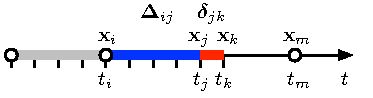
\includegraphics[width=0.6\textwidth]{figures/delta_time}
    \caption{The pre-integrated delta $\bfDelta_{ij}$ contains all motion from the last KF at time $i$, up to time $j$. 
    The current delta $\bfdelta_k$ contains the motion from times $j$ to $k$, computed from the last IMU measurement at time $k$.}
    \label{fig:delta_time}
\end{figure}

We perform pre-integration incrementally as follows. 
First, $\ol\bfDelta_{ii}$ is initialized to the null motion. 
Its covariance $\Cov_\Delta^{ii}$ and the Jacobian $\mjac{\bm\delta_i}{\bfb_i}$ are set to zero. 
At each reception of sensor data $\tilde\bfz_k$ at $t_k$, we integrate during $\dt$ to obtain the delta corresponding to a single data sample
%
\begin{equation}
    \bm\delta_k = f(\tilde\bfz_k, \ol\bfb_i, \dt)~, 
    \label{eq:data2delta}
\end{equation}
%
using the bias $\ol\bfb_i$ available in KF $i$. 
This single delta is integrated onto the delta pre-integrated so far using the delta composition law
%
\begin{equation}
    \ol\bfDelta_{ik} = \ol\bfDelta_{ij} \circ \bm\delta_k~. 
    \label{eq:deltaPlusDelta}
\end{equation}
%
which is represented in figure \figRef{fig:delta_time}.
%with Jacobians $\mjac{\ol\bfDelta_{ik}}{\ol\bfDelta_{ij}}$ and $\mjac{\ol\bfDelta_{ik}}{\bm\delta_k}$. 
The Jacobian of the pre-integrated delta with respect to biases, as well as the delta covariance, are also pre-integrated
%
\begin{align}
    \mjac{\bfDelta_{ik}}{\bfb_i} &= \mjac{\bfDelta_{ik}}{\bfDelta_{ij}}\mjac{\bfDelta_{ij}}{\bfb_i} 
+ \mjac{\bfDelta_{ik}}{\bm\delta_k}\mjac{\bm\delta_k}{\bfb_i} \\
    \Cov_\Delta^{ik} &= \mjac{\bfDelta_{ik}}{\bfDelta_{ij}}\Cov_\Delta^{ij}\mjac{\bfDelta_{ik}}{\bfDelta_{ij}}\tr 
+ \mjac{\bfDelta_{ik}}{\bm\delta_k}\mjac{\bm\delta_k}{\bfz_k}\Cov_\bfz\mjac{\bm\delta_k}{\bfz_k}\tr\mjac{\bfDelta_{ik}}{\bm\delta_k}\tr,
\end{align}
%
where $\mjac{\bm\delta_k}{\bfb_i}$, $\mjac{\bm\delta_k}{\bfz_k}$, $\mjac{\bfDelta_{ik}}{\bfDelta_{ij}}$ and $\mjac{\bfDelta_{ik}}{\bm\delta_k}$ 
are the Jacobians $\mjac{y}{x}=\partial y/\partial x$ of (\eqRef{eq:data2delta},\eqRef{eq:deltaPlusDelta}), computed according to Lie theory \cite{sola2018micro}, to which we give a brief introduction in \secRef{sec:lie_groups}.


\subsection{Residual definition}
\label{sec:preint_residual}

The pre-integrated $\ol\bfDelta_{im}$ is used at the end of the pre-integration to define the residual:

\begin{align}
    \bfe_{im}(\bfx^i, \bfx^m, \bias^i) = (\ol\bfDelta_{im} \oplus \mjac{\bfDelta_{im}}{\bfb_i}(\bfb_i-\ol\bfb_i) ) \ominus \hat\bfDelta_{im}
    \label{eq:preint_residual}
\end{align}
%
where $\bfb_i$ is the current bias value,  $\hat\bfDelta_{im}=\bfx^m\boxminus\bfx^i$ is the expected delta between KFs, and $\{\op,\om\}$ are the composite
 plus and minus operators described in section \secRef{sec:manifold_structure}. 
That is, $\{\op,\om\}$ are $\{+,-\}$ for vectors, and for rotations we have $\bfR\op\bm\theta\te\bfR\Exp(\bm\theta)$ and $\bfR_2\om\bfR_1\te\Log(\bfR_1\tr\bfR_2)$. 
The residual clearly depends on the KF states $\bfx^i,\bfx^m$ and the bias $\bfb_i$. It has an associated covariance  $\Cov_\Delta^{im}$.



\subsection{IMU pre-integration on Lie groups}

Let us come back to the IMU pre-integration problem defined in \secRef{sec:imu_preint_motivation}.
The states involved in this integration are the base states $\bfx = [\posi{}{}, \bfv, \Rot{}{}]$ with deltas $\bfDelta=[\Dp,\Dv,\DR]$. 
The IMU produces biased and noisy measurements $\tilde\bfz = [\tilde\bfa, \tilde{\bfomega}]$ of the base proper acceleration and angular velocity, 
with bias $\bfb = [\bias_{a}, \bias_{\omega}]$ and noise $\noise = [\noise_{a}, \noise_{\omega}]$. 

The pre-integration method in  \cite{forster2017-TRO} can be put in the formalism above by realizing that defining 
$\bm\delta=f(\tilde\bfz,\bfb,\dt)$ in \eqRef{eq:data2delta} as:
%
\begin{align}
    \bm\delta^k = \begin{bmatrix}
    \delta\bfp\\\delta\bfv\\\delta\bfR
    \end{bmatrix}^k =
    \begin{bmatrix}
    \tfrac12(\tilde\bfa-\bfb_a-\noise_a)\dt^2 \\
    (\tilde\bfa-\bfb_a-\noise_a)\dt \\
    \Exp((\tilde{\bfomega}-\bfb_\omega-\noise_\omega)\dt)
    \end{bmatrix}^k
\end{align}
%
and the composition law $\bfDelta^{ik}=\bfDelta^{ij}\circ\bm\delta^k$ in \eqRef{eq:deltaPlusDelta} as
%
\begin{align} \label{eq:composition_delta}
    \begin{split}
    \Dp^{ik} 
    &= \Dp^{ij} + \Dv^{ij}\dt + \DR^{ij}\dpp^{k} \\
    \Dv_{ik} 
    &= \Dv^{ij} + \DR^{ij}\dv^{k} \\
    \DR^{ik} 
    &= \DR^{ij}\dR^{k} 
    \end{split}
\end{align}

Then, $\bfx_k=\bfx_i\boxplus\bfDelta_{ik}$ is \cite[eq.~32]{forster2017-TRO} and $\bfDelta_{ik}=\bfx_k\boxminus\bfx_i$ is \cite[eq.~33]{forster2017-TRO}. 
Full details can be found in \cite[Section 3.4]{atchuthan-18-thesis}.



%
%
%
%
\section{IMU pre-integration on Lie groups}
In \cite{fourmy2019absolute}, we showed that an alternative formulation of IMU preintegration on Lie groups was possible.
We introduce a new matrix Lie group representation of the IMU deltas. The complete IMU pre-integration theory,
including the computation of the residual, is based on this new Lie structure. The theoretical material for the Lie
development in this section can be found in the report \cite{sola2018micro}.

\subsection{Lie Group formulation}

We propose a matrix form of the Lie group of IMU deltas as,
%
\begin{align}\label{equ:delta_Lie}
\D &= 
\begin{bmatrix}
\DR & \Dv & \Dp \\
\bf0 & 1 & \Dt \\
\bf0 & 0 & 1
\end{bmatrix} \in \cD \subset \bbR^{5\times 5}
~.
\end{align}

Group identity, inverse and composition stem from regular matrix identity, inverse (with $\DR\inv=\DR\tr$) and product,

\begin{align}
\D_\cE&=\begin{bmatrix}
\bfI & \bf0 & \bf0 \\
\bf0 & 1 & 0 \\
\bf0 & 0 & 1 
\end{bmatrix} = \bfI_{5\times5}
\label{equ:identity}
\\
\D\inv &= \begin{bmatrix}
\DR\tr & -\DR\tr\Dv & -\DR\tr(\Dp-\Dv\Dt) \\
\bf0 & 1 & -\Dt \\
\bf0 & 0 & 1
\end{bmatrix} 
\label{equ:inverse}
\\
\D\cdot\bm\delta 
&= 
\begin{bmatrix}
\DR\dR & \Dv + \DR\dv & \Dp+\Dv\dt + \DR\dpp \\
\bf0 & 1 & \Dt+\dt \\
\bf0 & 0 & 1
\end{bmatrix}
~.
\label{equ:composition}
\end{align}
%
% Comparing against \eqsRef{equ:composite_identity}{equ:composite_composition} we observe that this matrix Lie group is exactly equivalent to the classical IMU deltas above.



\subsubsection{Lie algebra \texorpdfstring{$\mathfrak{d}$}{d} and exponential map}

The Lie algebra elements $\bftau\hhat$ and their isomorphic Cartesian $\bftau$ have the forms
%
\begin{align}\label{equ:lie_algebra}
    \bftau\hhat &= \begin{bmatrix}
    \hatx{\bth} & \bfrho & \bfupsilon \\
    \bf0 & 0 & \Dt \\
    \bf0 & 0 & 0
    \end{bmatrix} \in \mathfrak{d}
    ,&
    \bftau &= \begin{bmatrix}
    \bfrho \\ \bfupsilon \\ \bth \\ \Dt
    \end{bmatrix}
    \te \begin{bmatrix}
    \bfv\Dt \\ \bfa\Dt \\ \bw\Dt \\ \Dt
    \end{bmatrix} 
    \in \bbR^{10}
    ,
\end{align}
%
with $\bfv\te\dot\Dp$, $\bfa\te\dot\Dv$ and $\hatx{\bw}\te\DR\tr\dot\DR$.
Operators $\wedge$ and $\vee$ are defined so that $\bftau\hhat=(\bftau)\hhat$ and $\bftau=(\bftau\hhat)\vvee$.

The exponential map transfers tangent elements to the group; the logarithmic map is its inverse,
%
\begin{align}
    \D &= \Exp(\bftau) \te \exp(\bftau\hhat) = \begin{bmatrix}
    \Exp(\bth) & \bfQ\bfupsilon & \bfQ\bfrho+\bfP\bfupsilon\Dt \\
    \bf0 & 1 & \Dt \\
    \bf0 & 0 & 1
    \end{bmatrix} %\in\cD 
    \label{equ:exp}
    \\
    \bftau &= \Log(\D) \te \log(\D)\vvee = \begin{bmatrix}
    \bfQ\inv(\Dp-\bfP\bfQ\inv\Dv\Dt) \\
    \bfQ\inv\Dv \\
    \Log(\DR) \\
    \Dt 
    \end{bmatrix} %\in \bbR^{10}
    \label{equ:log}
\end{align}
%
where $\Log()$ is obtained by identifying terms in \eqRef{equ:delta_Lie} and \eqRef{equ:exp}.
Matrices $\bfP$ and $\bfQ$ are provided in the appendix's \secRef{sec:IMULieGroup}.


\subsubsection{Jacobians, uncertainty}
\label{sec:uncertainty}

For general functions $f:\cM\to\cN;y=f(x)$, we propagate uncertainty normally via the Jacobians $\mjac{y}{x}\te\dpar{y}{x}$, \ie, $\Cov_y=\mjac{y}{x}\,\Cov_x\,\mjac{y}{x}\tr$. 
These Jacobians map the tangent spaces of the mannifolds $\cM,\cN$ at $x$ and $y$, and in case of vector spaces they resort to the classical Jacobian.
They also satisfy the chain rule, which we use extensively in our developments.
We provide ample reference and justification of this approach in the technical report \cite{sola2018micro}.

A comment is however necessary for the present IMU case.
It relates to the uncertainty of the last component of the tangent space \eqRef{equ:lie_algebra}, which is the time $\Dt$. This component has no uncertainty by definition. 
Having it in the covariances would imply singularity and result in the risk of a number of well-known numerical issues. 
We therefore systematically marginalize this time component out of the covariances, simply by removing the last row and column. 



\subsubsection{Delta Lie group IMU factor residual}
Computation of the residual in the case of the Lie Delta group formulation follows the steps defined in \secRef{sec:general-preint}.
However, since the Delta is directly defined as a Lie group, the formulation is actually simplified because  ... 
Use the pre-integrated Jacobian $\mjac{\D_{im}}{\bfb}$ to correct the pre-integrated delta $\ol\D_{im}$ to account for the new bias estimate $\bfb_i\neq\ol\bfb_i$,

\begin{align}
    \D_{im}(\bfb_i) &= \ol\D_{im}\cdot\Exp(\mjac{\D_{im}}{\bfb}(\bfb_i-\ol\bfb_i)) 
    ~.
\end{align}

Use \eqRef{equ:delta} as $\boxminus$ to compute the expected delta from  $\bfx_i$ to $\bfx_m$,

\begin{align}
    \widehat\D_{im}(\bfx_i,\bfx_m) &= \bfx_m \boxminus \bfx_i 
    ~.
\end{align}

Compute the residual in the  tangent of $\cD$ at $\D_{im}$,

\begin{align}
    \bfr^\Delta_{im}(\bfx_i,\bfx_m,\bfb_i) &= \Log(\D_{im}(\bfb_i)\inv \cdot \widehat\D_{im}(\bfx_i,\bfx_m)) \in \bbR^9
~,
\end{align}
%
and drop the $\Dt$ part from the residual after the $\Log()$ ---see comment in \secRef{sec:uncertainty}.
In this last equation, the composite minus operator $\oplus$ is simply the traditional Lie group "minus" operator defined in \cite{sola2018micro} applied
between the corrected preintegration delta and the expected delta.



\subsection{IMU Lie group versus Forster's method}

Mathematically, and disregarding methodology, the main difference between our method and Forster's \cite{forster2017-TRO} is to be found in the exponential map. 
To see it, let us consider small rotation increments $\bth=\bw\dt$ captured at each single IMU sample. 
In such cases, the matrices $\bfP,\bfQ$ appearing in the exponential map \eqRef{equ:exp} and detailed in \eqRef{equ:RQP} can be approximated by $\bfP\approx\tfrac12\bfI$ and $\bfQ\approx\bfI$.
The exponential becomes,
%
\begin{align}
    \Exp\left(\begin{bmatrix}
    \bf0 \\ \bfa \\ \bw \\ 1
    \end{bmatrix}\dt\right) \approx \begin{bmatrix}
    \Exp(\bw\dt) & \bfa\dt & \tfrac12\bfa\dt^2 \\
    \bf0 & 1 & \dt \\
    \bf0 & 0 & 1
    \end{bmatrix}
~,
\end{align}
%
where we find the terms $\bfa\dt$ and $\tfrac12\bfa\dt^2$, which should sound familiar from Forster's method. 
In effect, with this approximation, if we now compact all the steps \eqsRef{equ:pre_calibration}{equ:pre_composition} of our integration into a cumulative expression,
%
\begin{align}
    \D_{ik} = \prod_{j=i+1}^k \Exp\left(\begin{bmatrix}
    \bf0 \\ (\bfa_j-\bfa_{bi}) \\ (\bw_j-\bw_{bi}) \\ 1
    \end{bmatrix}\dt\right)
~,
\end{align}

It is possible (although tedious) to show that both Forster's and our method are exactly equivalent when $\bw\dt\to0$.
% , which is usually a valid hypothesis.
% These differences should not constitute an argument against Forster, since in practice we typically have extremely small steps $\bw\dt$ and the approximation holds very well.




\section{Related works}

Pre-integration principles were first proposed by Lupton \cite{lupton-09} to be applied to a smoothing based visual inertial estimator. His work was motivated partly 
by the fact that previous systems required a precise initialization of position, orientation and velocity (using a specialized routine) to begin to integrate IMU measurements. 
With this new formulation, Lupton noted that pre-integration of IMU measurements permitted to use measurements immediately and delay initial orientation about the gravity
vector in particular. 
This seminal work was quickly adopted by other authors using smoothing filters \cite{carlone2014eliminating}. As pioneering as this work was, it was however 
limited by the use of Euler angles whose problematic geometric properties are notorious. Indelman \cite{Indelman-2013-7768} first proposed to use the exponential of the 
matrix rotation group instead of Euler integration and to relax the assumptions of a non-rotating and flat earth of Lupton \cite{lupton-09}. Forster \cite{forster2015imu, forster2017-TRO}
proposed the same formulation using instead quaternions. Various experiments brought to light three main problem with the Euler angle formulation, that are completely absent 
from the quaternion "on-manifold" formulation. Firstly, first order integration of angular velocities using Euler angles is approximate, which leads to accumulated errors 
for high angular velocities or sampling rate.  Secondly, the log-likelihood of the angular displacement is not invariant under the action of rigid body transformations, 
\eg the choice of the world frame influence the results of the estimation. Finally, the well known gimbal lock singularity of Euler angles has a consequence 
on the covariance IMU noise covariance propagation, which is severely degraded when the robot trajectory comes close to the singularity. 
\cite{shen2015tightly}, later improved in \cite{qin2018vins} proposed to use a more precise numerical integration procedure than the default forward Euler used by Forster. 
Eckenhoff \cite{eckenhoff2019closed} derived closed form solutions of the preintegration equations using various piecewise constant models.

Barrau \cite{barrau2020mathematical} described a coupled matrix Lie group for the propagation of preintegration errors taking into account the earth rotation for aerospace
inertial navigation system in view. This work was later extended \cite{brossard2021associating} and showed that the linearized bias update is slightly more precise than 
the work of Forster \cite{forster2017-TRO}. Le Gentil \cite{le2020gaussian} used a different trajectory parametrization framework by formulating the preintegration algorithm 
in the context of Gaussian Process smoothing. Self calibration of IMU/Camera time offsets was also developped \cite{yang2020analytic}. 
\cite{luo2021unified} derived a comprehensive collection of motion models depending on the various possible choices of reference frames and motion conditions. 

As we saw the preintegration theory began in the context of visual-inertial odometry. It was however adapted to other high rate sensors such wheel odometry \cite{quan2019tightly}, 
possibly including self-calibration \cite{deray-19-selfcalib}. In his thesis, Atchuthan (\cite{atchuthan-18-thesis}, Section 4.3) derived the general form of the preintegration 
equations as a sensor agnostic form that is integrated in state estimation WOLF \cite{sola2021wolf}. As previously mentioned, other team applied preintegration theory in the 
context of factor graph legged robot state estimation to derive new leg odometry factors \cite{hartley2018legged, wisth2019robust, wisth2020preintegrated}.


